\documentclass[11pt,letterpaper]{article}

\usepackage{graphicx}

\usepackage{multicol}
\usepackage[margin=15mm]{geometry}

\usepackage{sidecap}
\sidecaptionvpos{figure}{c}


% define new environments
\usepackage{amsthm}
\theoremstyle{definition}
\newtheorem*{hypothesis}{Hypothesis}
\newtheorem*{objective}{Objective}

% per-section figure numbering
\usepackage{chngcntr}
\counterwithin{figure}{section}
% use dash instead of dot and use arabic section numbering
\renewcommand{\thefigure}{\arabic{section}-\arabic{figure}}

% use roman number formatting for sections
\renewcommand\thesection{\Roman{section}}

% disable subsection numbering
\setcounter{secnumdepth}{1}

\usepackage[super,sort&compress]{natbib}

% define multiple reference lists
\usepackage{multibib}
\newcites{self,own,ref}{Refereed publications in thesis,Other refereed publications,References}


% emphasize author name
\newcommand{\emphname}[1]{\underline{\textbf{#1}}}

\begin{document}

\begin{titlepage}

\setlength{\topmargin}{30mm}

\begin{center}
 
\textsc{\Large Committee meeting report}\bigskip

{\huge \bfseries Clinical genomics of medulloblastoma molecular subgroups}\\[10mm]

\begin{minipage}{0.6\textwidth}
\begin{multicols}{2}
	\begin{flushleft}
		\large \emph{Student:}\\
		David J. H. \textsc{Shih}
	\end{flushleft}
	\vfill
	\columnbreak
	\begin{flushright}
		\large \emph{Supervisors:}\\
		Dr.~Michael D. \textsc{Taylor}\\
		Dr.~Gary \textsc{Bader}\\
	\end{flushright}
	\begin{flushright}
		\large \emph{Committee:}\\
		Dr.~Meredith \textsc{Irwin}\\
		Dr.~Quaid \textsc{Morris}
	\end{flushright}
\end{multicols}
\end{minipage}

\vspace{20mm}

{ \large 
\textbf{Janurary 21, 2014}\\
\medskip
Peter Gilgan Centre for Research and Learning\\
686 Bay St\\
13th floor, Room 13.9701
}

\vspace{40mm}

\begin{flushleft}
	{ \large
	\textbf{Start date:} Janurary 3, 2011\\
	\textbf{Last meeting date:} April 24, 2012\\
	\medskip
	\textbf{Course requirements:} Complete\\
	\medskip
	\textbf{Refereed publications in thesis:} 3\\
	\textbf{Other refereed publications during program:} 13\\
	\textbf{Total refereed publications during program:} 16\\
	}
\end{flushleft}


\end{center}

\end{titlepage}


\clearpage

\bibliographystyleself{nature}
\bibliographyself{self}
\bigskip
$^*$ These authors contributed equally.

\clearpage

\bibliographystyleown{nature}
\bibliographyown{shih}

\clearpage

\section*{Summary of progress}

\nociteself{shih14,shih12,northcott12}

All aims have been completed. Aims I and II are published \citeself{northcott12,shih12}. Aim III is in press\citeself{shih14}.

\nociteown{ramaswamy13,remke13,dey13,markant13,natarajan13,zhukova13,dubuc13,diaz12,jones12,wu12,rausch12,dubuc12,northcott11}

\section*{Overview}

Medulloblastoma is the most common solid childhood malignancy \citeref{mainprize00}. Current therapy for medulloblastoma --- including surgical resection, radiation of the entire brain and spinal cord, and aggressive chemotherapy --- yields five-year survival rates of 60-70\% \citeref{gajjar06}. Survivors are often left with significant neurological, intellectual, and physical disabilities secondary to the effects of these non-specific, cytotoxic therapies on the developing nervous system \citeref{spiegler04,mabbott05}.

Recent evidence suggests that medulloblastoma in fact comprises a group of biologically distinct molecular entities whose clinical and genetic differences may require separate therapeutic strategies \citeref{thompson06,kool08,northcott11a,remke11,cho11}. Four principal subgroups\citeref{taylor12} of medulloblastoma have been identified: WNT, SHH, Group~3, and Group~4, and there is preliminary evidence for clinically significant subdivisions of the subgroups \citeref{northcott11a,cho11,remke11,taylor12,northcott11b}. Targeted therapies based on the genetics of the disease are not currently in use. However, inhibitors of the Sonic Hedgehog (Shh) pathway activator, Smoothened, have shown some early evidence of efficacy \citeref{rudin09}. With a deeper understanding of the genomics and biology of medulloblastoma subgroups, we hope to herald a new era of medulloblastoma treatment based on selective, specific, targeted therapy.

My study will focus on the following three obstacles that hinders the development of targeted therapy against medulloblastoma molecular subgroups:

\begin{enumerate}
	\item The lack of a clinically applicable assay for molecular subgrouping of medulloblastoma.
	\item The paucity of actionable targets for WNT, Group~3, and Group~4 medulloblastomas.
	\item Clinical trials of targeted therapy proceed without confirmed identifications of molecular targets in recurrent medulloblastomas.
\end{enumerate}

The objectives of my study are to provide viable solutions to these issues and to demonstrate the clinical significance of molecular classification.

\subsection{Aim I: Molecular classification of medulloblastoma in clinical contexts}

Although the retrospective classification of medulloblastoma has been scientifically informative, molecular subgrouping has not been applied in the context of a prospective clinical trial. One major obstacle is the lack of fresh-frozen samples for most clinical cases. Expression profiling, on which molecular classification was based, depends on the availability of high-quality RNA. In contrast, clinical samples are routinely subjected to formalin-fixation and paraffin-embedding (FFPE), which preserves tissue integrity but causes nucleic acid degradation. To facilitate the development of therapy specifically targeted against molecular subgroups, we sought to establish an molecular subgrouping assay that can be clinically applied on FFPE samples. In collaboration with Paul Northcott, I established a simple analytic pipeline to molecular subgrouping using expression data generated by nanoString assays, and demonstrated its high classification accuracy on FFPE samples \citeself{northcott12}.

\subsection{Aim II: Target identification by copy-number profiling of medulloblastoma}

After having established a clinically applicable molecular classification methodology, I turned to the problem of identifying molecular targets in medulloblastoma. Unlike SHH medulloblastomas, actionable targets for WNT, Group~3, and Group~4 tumours have yet been identified. However, prior attempts may have been underpowered to discriminate the genomic differences among the four molecular subgroups. To this end, the Medulloblastoma Advanced Genomics International Consortium (MAGIC), consisting of scientists and physicians from 43 cities across the globe, has gathered $>1200$ medulloblastomas. Paul Northcott and I have analyzed the genomic copy-number profiles of the tumours by Single Nucleotide Polymorphism (SNP) arrays. We have identified genes and pathways that characterize each medulloblastoma subgroup \citeself{shih12}.

\subsection{Aim III: Demarcating the genomic differences between primary and recurrent tumours}

To date, most clinical efforts and changes in pediatric tumour treatment has been in the optimization of chemotherapy and radiation protocols \citeref{bouffet10}. While survival rates for medulloblastoma patients have improved over the years, patients with recurrent medulloblastoma currently have no effective treatment option. These patients are often enrolled in clinical trials based on diagnostic tests of their primary disease, under the likely erroneous assumption that recurrent tumours are identical to their primary counterparts. As MAGIC has collected one of the largest set of matched primary-recurrent medulloblastomas, I will analyze these tumours by copy-number profiling and Whole-Genome Sequencing (WGS). From the data, I will identify the genomic differences between primary and recurrence and establish their biological significance.

\clearpage


\section{Molecular classification of medulloblastoma in clinical contexts}

\begin{objective}
To develop a clinically applicable assay for molecular classification of medulloblastoma.
\end{objective}

The nanoString nCounter technology \citeref{geiss08} was used to directly measure the expression level of 22 medulloblastoma subgroup specific signature genes. The nanoString assay directly interrogates nucleic acid levels without polymerase chain reaction (PCR) amplification (or other enzymatic reactions) in multiplexed system, using pairs of fluorescent probes that bind to target sequences. We developed an analytic method that can accurately predict molecular subgroups of medulloblastoma, even on archival FFPE samples \citeself{northcott12}.

A set of widely used classifiers were trained using a training set of 101 medulloblastomas with known subgroup affiliations. The classifiers were tuned and assessed using cross-validation. The most accurate classifier (across all tested accuracy measures) was selected for classification.

The assay was validated on an external set of 130 non-overlapping medulloblastomas, and it achieved an accuracy of 98\% (\textbf{Figure~\ref{fig:nanostr-valid}}). Further, the assay yielded reproducible predictions when repeated in three independent laboratories \citeself{northcott12}. The clinical applicability of the assay was demonstrated by its predictive accuracy on FFPE samples of archival ages $\leq 8$ years (\textbf{Figure~\ref{fig:nanostr-ffpe}}). The accuracy decreased on older FFPE samples, presumably due to poorer RNA integrity, though standard measurements of RNA quality were not correlated with accuracy \citeself{northcott12}.

Above all, a rapid, reliable, and reproducible assay was developed for assigning molecular subgroups to clinical samples, available as frozen or recent FFPE material, and this assay is highly suited for future medulloblastoma clinical trials.

\clearpage

\begin{figure}[h]
	\begin{center}
		\includegraphics[width=\textwidth]{fig/nanostr-class/nanostr-valid.pdf}
	\end{center}
	\caption{Validation of classification assay on independent medulloblastoma cohorts.}
	\textbf{a-c}, Expression heatmaps of nanoString class-predicted medulloblastomas of known subgroup status as published by Remke et al.\citeref{remke11} (a), Cho et al.\citeref{cho11} (b), and Kool et al.\citeref{kool08} (c). Samples are sorted according to subgroup predictions. Known expression subgroup affiliations and erroneously classified cases are marked above the heatmap. \textbf{d}, \emph{Left}, Pie chart depicting the known subgroup distribution of medulloblastomas from the three independent cohorts analyzed in \textbf{a-c} ($n = 130$) and the subgroups predicted by nanoString profiling. Misclassified cases are marked within each slice according to the predicted subgroups. \emph{Right}, Pie chart of class prediction accuracy ($127/130$) from the validation set. Adapted from Northcott et al.\citeself{northcott12}
	\label{fig:nanostr-valid}
\end{figure}

\begin{figure}[h]
	\begin{center}
		\includegraphics[width=\textwidth]{fig/nanostr-class/nanostr-ffpe.pdf}
	\end{center}
	\caption{Classification performance on formalin-fixed paraffin embedded (FFPE) archival samples.}
	\textbf{a}, Class prediction accuracy in relation to sample age of archival medulloblastomas stored as FFPE material ($n = 84$). Samples obtained within the past 8 years exhibit accuracies of $\geq 95\%$, as demarcated by the red vertical line. \textbf{b}, Heatmap of nanoString data showing class predictions for FFPE cases of $\leq 8$ years confidently predicted by the assay ($n = 28$). Samples are sorted according to subgroup prediction. All cases satisfying prediction probability threshold were assigned to the correct subgroup ($28/28$). Adapted from Northcott et al.\citeself{northcott12}
	\label{fig:nanostr-ffpe}
\end{figure}

\clearpage

\section{Target identification by copy-number profiling of medulloblastoma}

\begin{hypothesis}
Each medulloblastoma molecular subgroup is characterized by specific genomic aberrations.
\end{hypothesis}

Copy-number profiles were generated on $> 1200$ medulloblastomas using the Affymetrix Genome-wide SNP6 platform. After quality control and clinical criteria filtering, copy-number profiles of $1087$ primary medulloblastomas were available for further analysis in identifying somatic copy-number aberrations (SCNAs): regions of aberrant gains and losses in the tumour genome. The tumours were stratified based on molecular subgroups, as determined by the method described in \textbf{Aim 1}. The copy-number and cytogenetic profiles of medulloblastoma subgroups were highly divergent, demonstrating that medulloblastoma subgroups are genomically heterogeneous (\textbf{Figure~\ref{fig:cn-heatmap}--\ref{fig:broad-events}}). Indeed, when the cohort was analyzed by each subgroup independently, an increased number of SCNAs were identified, many of which were subgroup-enriched (\textbf{Figure~\ref{fig:subgroup-specificity}}).

Among the recurrent high-level amplifications (copy-number $\geq 5$) identified (\textbf{Figure~\ref{fig:high-level-amps}}), the most prevalent events targeted members of the MYC family (\emph{MYCN}, \emph{MYC}, \emph{MYCL1}), with \emph{MYCN} predominantly amplified in SHH and Group~4, \emph{MYC} in Group~3, and \emph{MYCL1} in SHH medulloblastomas.
The most common homozygous deletions targeted known tumour suppressors \emph{PTEN}, \emph{PTCH1}, and \emph{CDKN2A/B}, all of which were enriched in SHH tumours (\textbf{Figure~\ref{fig:homo-del}}). A selected set of genes were assessed using custom nanoString assays, and 90.9\% of events were verified (\textbf{Figure~\ref{fig:nanostr-verification}}). Additional genes were validated on external cohorts by interphase fluorescence \emph{in situ} hybridization (\textbf{Figure~\ref{fig:mdm4-fish},~\ref{fig:acvr2b-fish}}).

The disparate genomic landscapes of medulloblastoma subgroups lead to the identification of a multitude of focal SCNAs that characterize each molecular subgroup (\textbf{Figure~\ref{fig:shh-gistic},~\ref{fig:group3-gistic},~\ref{fig:group4-gistic}}). Novel genes identified in this study include: \emph{PPM1D}, \emph{PIK3C2B}, and \emph{MDM4} in SHH (\textbf{Figure~\ref{fig:shh-amps-igv}}); \emph{ACVR2A}, \emph{ACVR2B}, and \emph{TGFBR1} in Group~3 (\textbf{Figure~\ref{fig:group3-amps-igv}}); and \emph{NFKBIA} and \emph{USP4} in Group~4 (\textbf{Figure~\ref{fig:group4-dels-igv}}). Conversely, WNT medulloblastoma have few recurrent SCNAs (\textbf{Figure~\ref{fig:genome-coverage}}). 

SHH medulloblastoma, which is characterized by activation of Shh signaling\citeref{northcott11a,remke11,cho11,kool08,taylor12}, exhibit frequent SCNAs in the Shh pathway. Genes involved in focal SCNAs amplifications are significantly associated with SHH medulloblastoma signatures genes (\textbf{Figure~\ref{fig:shh-signature}}), suggesting that copy-number changes contribute in part to the altered expression signatures previously observed in SHH tumours. Accordingly, positive regulators of Shh signaling (\emph{MYCN} and \emph{GLI2}) were recurrently amplified, while a negative regulator of Shh signaling (\emph{PTCH1}) was recurrently lost. Consistent with their functions in the same pathway, these events were mutually exclusive; however, they lead to different clinical outcomes (\textbf{Figure~\ref{fig:shh-me}}). In additional to Shh signaling, other core pathways recurrently disrupted in SHH medulloblastoma are TP53 signaling and RTK/PI3K signaling (\textbf{Figure~\ref{fig:shh-pathways}}).

The signaling pathways involved in Group~3 and Group~4 medulloblastomas are less well understood, as suggested by their names. Nonetheless, at the copy-number level, distinct pathways were dysregulated in Group~3 and Group~4 (\textbf{Figure~\ref{fig:group3-vs-group4}}). Group~3 tumours are characterized by amplification of \emph{MYC} and \emph{OTX2}, which occur in a mutually exclusive pattern (\textbf{Figure~\ref{fig:group3-me}}). This observation is consistent with the tendency of the two oncogenic transcription factors to bind the same promoter regions \citeref{bunt11}. Further, the TGF$\beta$ signaling pathway is frequently disrupted by SCNAs in Group~3. Conversely, the NF-$\kappa$B pathway appear to genetically targeted in Group 4 medulloblastomas.

The most prevalent focal gain (and previously neglected) in Group~4 was the somatic tandem duplication of the \emph{SNCAIP} gene (\textbf{Figure~\ref{fig:sncaip-gain}}). SNCAIP expression is highly elevated in Group~4 medulloblastomas (\textbf{Figure~\ref{fig:sncaip-expr}}). In fact, \emph{SNCAIP} duplication is further restricted to the Group~4$\alpha$ and may play a functional role in this medulloblastoma subtype (\textbf{Figure~\ref{fig:group4-alpha-beta}}). Another lab member, Vijay Ramaswamy, has begun functional characterization of this gene.

While \emph{MYC} amplification is a known pivotal player Group~3, our data indicated that others genes in close proximity to the \emph{MYC} locus may also play cooperative roles. This locus was frequently disrupted by a multitude of high-level amplicons (\textbf{Figure~\ref{fig:chromothr_myc}}) as well as massively genomic rearrangements (\textbf{Figure~\ref{fig:chromothr_myc_wgs}}). These genomic aberrations are reminiscent of chromothripsis (chromosome shattering), which has recently been implicated in cancer formation \citeref{stephens11,liu11,kloosterman11b,magrangeas11,crasta12,molenaar12}, as well as in medulloblastoma \citeself{rausch12}. As a consequence of these events, the adjacent \emph{PVT1} gene and miR-1204 are frequently co-amplified with \emph{MYC}. Moreover, amplifications of the \emph{MYC}/\emph{PVT1} locus frequently result in the formation of fusion transcripts. Concurrent with MYC-PTV1 fusion expression, miR-1204 (hosted in PTV1) is upregulated (\textbf{Figure~\ref{fig:myc-fusion_mir-expr}}). \emph{MYC}, \emph{PVT1}, and miR-1204 all have been previously shown to play independent functional roles in other tumours \citeref{guan07,carramusa07,huppi08,barsotti12}, and may synergistically promote tumourigenesis.

In summary, medulloblastoma subgroups are characterized by distinct genomic aberrations that dysregulated disparate signaling pathways. Importantly, the amplified genes and activated pathways identified in this study could serve as potential targets for therapeutic development in medulloblastoma subgroups.

\clearpage

\begin{SCfigure}
	\centering
	\includegraphics[width=0.6\textwidth]{fig/magic-cn/cn-heatmap.png}
	\caption{Genome-wide copy-number profile of medulloblastoma subgroups.
	Copy-number profiling was performed on 1087 non-overlapping primary medulloblastomas. Shown is a copy number heatmap for 827 cases classified according to medulloblastoma subgroup based on matched gene expression data.  Amplifications are shown in red and deletions in blue.}
	\label{fig:cn-heatmap}
\end{SCfigure}

\begin{SCfigure}
	\centering
	\includegraphics[width=0.6\textwidth]{fig/magic-cn/broad-events.pdf}
	\caption{Frequency and significance of broad cytogenetic events across medulloblastoma subgroups.
	Gains are plotted in red and deletions in blue, shaded according to significance ($q < 0.1$, binomial test).}
	\label{fig:broad-events}
\end{SCfigure} 


\clearpage

\begin{SCfigure}
	\centering
	\includegraphics[width=0.5\textwidth]{fig/magic-cn/subgroup-specificity.pdf}
	\caption{Significant regions of focal SCNA identified by GISTIC2 in pan-cohort or subgroup-stratified analyses.
	A total of 62 significant regions were identified when the cohort was analyzed as a single group, whereas 110 significant regions were captured when the cohort was analyzed according to subgroup. The number of significant subgroup-enriched regions identified more than doubled (73 vs. 30) when the subgroups were analyzed independently.}
	\label{fig:subgroup-specificity}
\end{SCfigure}

\begin{SCfigure}
	\centering
	\includegraphics[width=0.4\textwidth]{fig/magic-cn/genome-coverage}
	\caption{WNT medulloblastomas have a paucity of recurrent focal SCNAs. Bar-plots of the proportion of genome recurrently disrupted by focal SCNAs are depicted for each medulloblastoma subgroup.}
	\label{fig:genome-coverage}
\end{SCfigure}

\begin{SCfigure}
	\centering
	\includegraphics[width=0.7\textwidth]{fig/magic-cn/high-level-amps.pdf}
	\caption{Recurrent high-level amplifications in medulloblastoma.
	Frequency of genes amplified (segmented copy-number $\geq 5$) in at least two samples are shown with the distribution of the event across subgroups. The number of genes mapping to the peak region as defined by GISTIC2 (where applicable) are listed in parentheses after the candidate driver gene.}
	\label{fig:high-level-amps}
\end{SCfigure}

\begin{SCfigure}
	\centering
	\includegraphics[width=0.6\textwidth]{fig/magic-cn/homo-del.pdf}
	\caption{Recurrent homozygous deletions in medulloblastoma. Frequency of genes targeted by homozygous deletion (segmented copy-number $\leq 0.7$) in at least two samples are shown.}
	\label{fig:homo-del}
\end{SCfigure}

\begin{SCfigure}
	\centering
	\includegraphics[width=0.5\textwidth]{fig/magic-cn/nanostr-verification.pdf}
	\caption{Verification of focal SCNAs by nanoString.
	Genes inferred to be focally amplified by SNP6 were interrogated using a custom nanoString CodeSet across a set of 192 medulloblastomas selected from our cohort. Bar-plot shows the number of samples for which each gene is verified (red) or not (black). An overall verification rate of 90.9\% was achieved.}
	\label{fig:nanostr-verification}
\end{SCfigure}

\clearpage

\begin{figure}[h]
	\begin{center}
		\includegraphics[width=\textwidth]{fig/magic-cn/shh-gistic.pdf}
	\end{center}
	\caption{Landscape of SCNAs in SHH medulloblastoma.}
	GISTIC2 significance plot of amplifications (red) and deletions (blue) observed in the SHH subgroup is shown.
	Labeled cytobands indicate significant regions that satisfied multiple criteria to qualify as a potential somatic event. The number of genes mapping to each significant region are shown in parentheses next to the cytoband label.  Regions over-represented in SHH are highlighted in red.
	\label{fig:shh-gistic}
\end{figure}

\clearpage

\begin{SCfigure}
	\centering
	\includegraphics[width=0.4\textwidth]{fig/magic-cn/shh-signature.pdf}
	\caption{Significant overlap between SHH signature genes and genes targeted by focal SCNAs in SHH.
		Bar-plots show the overlap significance based on permutation tests between SHH signature genes reported in the Cho (\emph{left}) or Northcott (\emph{right}) studies and genes mapping to focal SCNAs in our dataset. Dashed line indicates significance threshold ($\alpha = 0.05$).}
	\label{fig:shh-signature}
\end{SCfigure}

\begin{SCfigure}
	\centering
	\includegraphics[width=0.5\textwidth]{fig/magic-cn/shh-amps-igv.pdf}
	\caption{Recurrent high-level amplifications of \emph{PPMID} and co-amplification of \emph{MDM4} and \emph{PIK3C2B} in SHH medulloblastoma.
	Segmented copy-number tracks are shown for the amplified loci (17q23 and 1q23).}
	\label{fig:shh-amps-igv}
\end{SCfigure}

\begin{SCfigure}
	\centering
	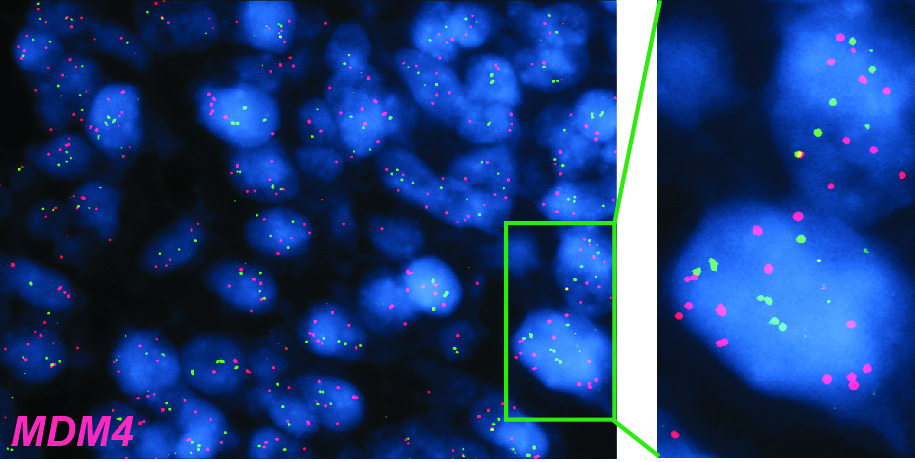
\includegraphics[width=0.4\textwidth]{fig/magic-cn/mdm4-fish.jpg}
	\caption{Validation of \emph{MDM4} amplification in medulloblastoma.
	Interphase fluorescence \emph{in situ} hybridization (FISH) of the \emph{MDM4} locus confirmed amplification in 8.2\% (12/146) of external cases present on a medulloblastoma tissue microarray (work by Andrey Korshunov).}
	\label{fig:mdm4-fish}
\end{SCfigure}

\clearpage

\begin{figure}[h]
	\begin{center}
		\includegraphics[width=\textwidth]{fig/magic-cn/shh-me.pdf}
	\end{center}
	\caption{Mutually exclusivity and clinical significance of focal SCNAs in SHH medulloblastomas.}
	Mutual exclusivity analysis of focal SCNAs in SHH medulloblastoma reveals that the most prevalent events in this subgroup do not co-occur in the same sample and collectively contribute to 23\% of cases, suggesting functional redundancy of SCNAs. Nevertheless, the mutually exclusive events exhibit distinct clinical outcome. Patients exhibiting either \emph{MYCN} or \emph{GLI2} amplification have poor clinical outcomes, while those exhibiting focal \emph{PTCH1} deletion have improved overall survival.
	\label{fig:shh-me}
\end{figure}

\begin{figure}[h]
	\begin{center}
		\includegraphics[width=\textwidth]{fig/magic-cn/shh-pathways.pdf}
	\end{center}
	\caption{Core pathways genetically targeted in SHH medulloblastoma.}
	Summary of SCNAs affecting components of Shh signaling, TP53 signaling, and RTK/PI3K signaling are depicted. Colours reflect the frequency by which the respective genes are targeted by focal or broad events in SHH medulloblastomas (red for amplification, blue for deletion). Significance values indicate the prevalence with which each pathway is targeted in SHH vs. non-SHH cases (Fisher's exact test).
	\label{fig:shh-pathways}
\end{figure}

\clearpage

\begin{figure}[h]
	\begin{center}
		\includegraphics[width=\textwidth]{fig/magic-cn/group3-gistic.pdf}
	\end{center}
	\caption{Landscape of SCNAs in Group~3 medulloblastoma.}
	GISTIC2 significance plot of recurrent amplifications and deletions in Group~3 is shown. Events highlighted in yellow are enriched in Group~3.
	\label{fig:group3-gistic}
\end{figure}

\clearpage

\begin{figure}[h]
	\begin{center}
		\includegraphics{fig/magic-cn/group3-me.pdf}
	\end{center}
	\caption{Mutual exclusivity of \emph{MYC}, \emph{OTX2}, and \emph{DDX31} aberrations in Group~3.}
	Analysis of focal SCNAs reveals that \emph{MYC} amplification and \emph{OTX2} amplification are completely mutually exclusivity, and these events are prognostic significant: \emph{MYC} amplified cases show poorer overall survival.
	\label{fig:group3-me}
\end{figure}

\begin{SCfigure}
	\centering
	\includegraphics[width=0.45\textwidth]{fig/magic-cn/group3-amps-igv.pdf}
	\caption{Recurrent amplifications target receptors of the TGF$\beta$ superfamily in Group~3.
		Segmented copy-number tracks of Group~3 medulloblastomas show recurrent high-level amplifications affecting \emph{ACVR2A} (2q22), \emph{ACVR2B} (3p22), and \emph{TGFBR1} (9q22).}
	\label{fig:group3-amps-igv}
\end{SCfigure}

\begin{SCfigure}[3.0]
	\centering
	\includegraphics[width=0.2\textwidth]{fig/magic-cn/acvr2b-fish.jpg}
	\caption{Validation of \emph{ACVR2B} amplification.
	FISH of the \emph{ACVR2B} locus confirmed presence of amplification in an external cohort of medulloblastomas on a TMA (work by Andrey Korshunov).}
	\label{fig:acvr2b-fish}
\end{SCfigure}

\begin{SCfigure}
	\centering
	\includegraphics[width=0.5\textwidth]{fig/magic-cn/group3-pathways.pdf}
	\caption{TGF$\beta$ signaling is recurrently disrupted by SCNAs in Group~3.
SCNAs affecting the TGF$\beta$ pathway comprise 20.2\% of Group~3 cases and are significantly enriched in Group~3 compared to non-Group~3 cases (Fisher’s exact test).}
	\label{fig:group3-pathways}
\end{SCfigure}

\clearpage

\begin{figure}[h]
	\begin{center}
		\includegraphics[width=\textwidth]{fig/magic-cn/group4-gistic.pdf}
	\end{center}
	\caption{Landscape of SCNAs in Group~4 medulloblastoma.}
	GISTIC2 significance plot of amplification and deletion regions in Group~4 is shown. Events highlighted in green are enriched in Group~4.
	\label{fig:group4-gistic}
\end{figure}

\clearpage

\begin{SCfigure}[2.0]
	\centering
	\includegraphics[width=0.3\textwidth]{fig/magic-cn/group4-dels-igv.pdf}
	\caption{NF-$\kappa$B pathway is recurrently targeted in Group~4.
		Recurrent focal deletions disrupt \emph{NFKBIA} and \emph{USP4}, negative regulators of the NF-$\kappa$B pathway, in Group~4 medulloblastoma.}
	\label{fig:group4-dels-igv}
\end{SCfigure}

\begin{SCfigure}
	\centering
	\includegraphics[width=0.5\textwidth]{fig/magic-cn/group3-vs-group4.pdf}
	\caption{Aberrations disrupt distinct pathways in Group~3 and Group~4 medulloblastomas.
	Enrichment plot of gene sets disrupted by SCNAs in Group~3 vs. Group~4 medulloblastomas.}
	\label{fig:group3-vs-group4}
\end{SCfigure}

\clearpage

\begin{figure}[h]
	\begin{center}
		\includegraphics[width=\textwidth]{fig/magic-cn/sncaip-gain.png}
	\end{center}
	\caption{Focal gains recurrently target \emph{SNCAIP} in Group~4.}
	\emph{Left}, Segmented copy-number tracks of 317 Group~4 tumours shows a highly recurrent region of focal gain at 5q23.2 targeting a single gene: \emph{SNCAIP}, observed in 10.4\% of Group~4 cases (33/137). Whole-genome sequencing confirms that \emph{SNCAIP} is tandemly duplicated\citeself{shih12}. \emph{Right}, Analysis of matched-germline confirms that \emph{SNCAIP} duplication is somatic.
	\label{fig:sncaip-gain}
\end{figure}

\begin{figure}[h]
	\begin{center}
		\includegraphics[width=\textwidth]{fig/magic-cn/sncaip-expr.pdf}
	\end{center}
	\caption{\emph{SNCAIP} is a Group~4 signature gene.}
	\emph{Left}, Box-plot depicting SNCAIP significant upregulation in Group~4 (Mann-Whitney test), as determined by expression analysis of a previously published cohort of 103 primary medulloblastoma \citeref{northcott11a}. SNCAIP ranks among the top 1\% of most highly expressed genes in Group~4 medulloblastoma (rank 39 out of 16758).
	\emph{Right}, Validation of SNCAIP as a Group~4 signature gene across five published medulloblastoma expression datasets: Thompson \citeref{thompson06}, Kool \citeref{kool08}, Fattet, Cho \citeref{cho11}, and Remke \citeref{remke11}. Expression datasets total 396 cases on four different array platforms. In all datasets, SNCAIP exhibited highest expression in Group~4.
	\label{fig:sncaip-expr}
\end{figure}

\begin{figure}[h]
	\begin{center}
		\includegraphics[width=\textwidth]{fig/magic-cn/group4-alpha-beta.pdf}
	\end{center}
	\caption{\emph{SNCAIP} duplication is restricted to one subtype of Group~4.}
	\textsf{a}, Non-negative matrix factorization (NMF) consensus clustering performed on expression profiles of Group~4 cases ($n = 188$) reveal two transcriptionally distinct subtypes of Group~4, designated $4\alpha$ and $4\beta$. SNCAIP duplicated is significantly enriched in the Group $4\alpha$ subtype (Fisher's exact test).
	\textsf{b}, SNCAIP expression is significantly elevated in Group $4\alpha$ compared to $4\beta$ (Mann-Whitney test).
	\textsf{c}, SNCAIP expression is copy number-driven in Group $4\alpha$. Group $4\alpha$ cases were stratified by \emph{SNCAIP} copy-number status. Samples harbouring SNCAIP duplication exhibit a significant \~1.5-fold increase in SNCAIP expression (Mann-Whitney test).
	\label{fig:group4-alpha-beta}
\end{figure}

\clearpage

\begin{figure}[h]
	\begin{center}
		\includegraphics[width=\textwidth]{fig/magic-cn/chromothr_myc_ai.pdf}
	\end{center}
	\caption{A multitude of amplicons disrupt the \emph{MYC}/\emph{PVT1} locus.}
	Copy-number plot of 8q24.21 is shown for a representative sample. Dots represent raw copy-number estimates and lines denote copy-number segments and state (red: gain, blue: loss). 71.4\% of \emph{MYC}-amplified (20/28) cases exhibit (partial) co-amplification of adjacent non-coding \emph{PVT1} gene and miR-1204. PVT1-MYC fusion transcripts were detected by RNA-seq, qRT-PCR, and Sanger sequencing in 8/20 samples \citeself{shih12}.
	\label{fig:chromothr_myc}
\end{figure}

\begin{figure}[h]
	\begin{center}
		\includegraphics[width=0.8\textwidth]{fig/magic-cn/chromothr_myc_wgs.pdf}
	\end{center}
	\caption{Chromothripsis disrupts the \emph{MYC}/\emph{PVT1} locus.}
	Whole-genome sequencing confirms a complex pattern of rearrangements on 8q24 in a representative sample, reminiscent of chromothripsis (chromosome shattering).
	Plot shows chromosome 8 copy-number estimates (derived from read depth ratio of tumour vs. matched germline).
	Complex rearrangements are observed in concordance with a multitude of amplicons in the 8q24 region.
	\label{fig:chromothr_myc_wgs}
\end{figure}

\begin{figure}[h]
	\begin{center}
		\includegraphics[width=0.6\textwidth]{fig/magic-cn/chromothr-enrich.pdf}
	\end{center}
	\caption{Chromothripsis frequently disrupt chromosome 8 in Group~3 medulloblastoma.}
	Quantification of inferred chromothripsis across medulloblastoma subgroups reveal a significant enrichment of chromothripsis on chromosome 8 in Group~3 ($q = 0.0004$, Fisher's exact test), as compared to the entire cohort. Samples exhibiting at least 10 copy-number state changes on a single chromosome were inferred to have undergone chromothripsis.
	\label{fig:chromothr-enrich}
\end{figure}

\begin{figure}[h]
	\begin{center}
		\includegraphics{fig/magic-cn/myc-fusion_mir-expr.pdf}
	\end{center}
	\caption{miR-1204 is upregulated in Group~3 cases harbouring PVT1-MYC fusions.}
	Quantitative RT-PCR analysis of microRNAs hosted by PVT1 confirms upregulation of miR-1204 in Group~3 cases harbouring PVT1-MYC fusions (Mann-Whitney test). Samples were categorized as MYC-balanced/fusion(-) ($n = 4$), MYC-amplified/fusion(-) ($n = 6$), or MYC-amplified/fusion(+) ($n = 8$). Expression of microRNAs in MYC-balanced/fusion(-) samples served as baselines for determining relative expressions of the respective microRNAs in the other groups. Experiments were performed by John Peacock.
	\label{fig:myc-fusion_mir-expr}
\end{figure}

\clearpage

\section{Demarcating the genomic differences between primary and recurrent tumours}

\begin{hypothesis}
Primary and recurrent medulloblastomas are genetically different, which may cause differential responses to therapy.
\end{hypothesis}

To delineate the genomic differences between primary and recurrent medulloblastoma, we performed a genome-wide copy-number profiling analysis on 21 pairs/sets of primary and recurrent samples, and compared the somatic copy-number aberrations of recurrent tumours to their matched primary. In $>80\%$ of cases, recurrent tumours have acquired additional alterations, have arisen from a cancer clone distinct from the dominant clone in the primary tumour, or appear to be \emph{de novo} tumours. Importantly, we found that recurrent tumours can ‘lose’ critical amplicons, such as \emph{MYCN} and \emph{GLI2}, which characterize the molecular subgroup of the primary tumours. Such genomic differences would likely lead to differential response to targeted therapy and impact the outcome of clinical trials. Currently, we are conducting whole-genome sequencing to bolster our observations from copy-number profiling.

Current clinical trials of targeted therapy in medulloblastoma involve target identification in the untreated primary tumour, followed by administration of the targeted therapy at the time of recurrence when the target may no longer be present. If our hypothesis is correct, this schema is a recipe for failure.  We propose that future clinical trials of targeted agents for recurrent medulloblastoma should mandate re-biopsy to ascertain the continued presence of the target, or the targeted agent should be used upfront on the untreated primary tumour.

\clearpage

\begin{multicols}{2}
\small
\bibliographystyleref{nature}
\bibliographyref{mb,tech,chromothr,cancer}
\end{multicols}


\end{document}

